% Copyright (c) Eclipse Arrowhead Project
%
% This program and the accompanying materials are made available under the
% terms of the Eclipse Public License 2.0 which is available at
% http://www.eclipse.org/legal/epl-2.0.
%
% SPDX-License-Identifier: EPL-2.0

\documentclass[a4paper]{arrowhead}

\usepackage[yyyymmdd]{datetime}
\usepackage{enumitem}
\usepackage{etoolbox}
\usepackage[utf8]{inputenc}
\usepackage{multirow}

\renewcommand{\dateseparator}{-}

\begin{document}

%% Arrowhead Document Properties
\ArrowheadTitle{X.509 Certificate Profiles}
\ArrowheadType{Profile Description}
\ArrowheadTypeShort{PD}
\ArrowheadVersion{1.0}
\ArrowheadDate{\today}
\ArrowheadAuthor{Emanuel Palm}
\ArrowheadOrganization{Eclipse Arrowhead}
\ArrowheadStatus{Proposal}
\ArrowheadContact{emanuel.palm@pinterop.se}
\ArrowheadAbstract{
  This document specifies how X.509 certificates are to be configured, issued and validated to facilitate secure identification and communication within and between \textit{Eclipse Arrowhead} local clouds, when such security is desired and the kind of certificate is relevant.
}
\ArrowheadFooter{\href{www.arrowhead.eu}{www.arrowhead.eu}}
\ArrowheadSetup
%%

%% Front Page
\ArrowheadFrontPage
%%

%% Table of Contents
\tableofcontents
\newpage
%%

\section{Introduction}
\label{sec:introduction}
% Copyright (c) 2021-10-07 Eclipse Arrowhead Project
%
% This program and the accompanying materials are made available under the
% terms of the Eclipse Public License 2.0 which is available at
% http://www.eclipse.org/legal/epl-2.0.
%
% SPDX-License-Identifier: EPL-2.0

We, the Eclipse Arrowhead project, here present and authoritative set of Arrowhead concept definitions, meant to serve as the foundational language for discussions about and the modelling of Arrowhead-based designs.
The document exists to help mitigate compatibility and consistency issues in software, tooling, models and all other things of relevance to Arrowhead.
The concepts established here are not specified in terms of any particular modelling tools or languages, but should be useful as foundation for any other Arrowhead modelling or documentation effort.

The description of Arrowhead we present here should be seen as an extension of \textit{Reference Architecture Model Industrie 4.0} (RAMI4.0) \cite{adolphs2016reference}.
This means that we take key concepts from RAMI4.0 and present them here in the context of the Arrowhead framework.
As RAMI4.0 is defined partly in terms of \textit{Service-Oriented Architecture} (SOA), we also builds upon \textit{Reference Model for Service Oriented Architecture} (SOA-RM) \cite{mackenzie2006reference}.
In other words, this document assumes a world-view of service-oriented communication in an Industry 4.0 setting.
This world-view is introduced more fully in Section \ref{sec:arrowhead}.

\subsection{Primary Audiences}
\label{sec:introduction:audiences}

This document is being written and maintained with the following primary audiences in mind:

\begin{itemize}
\item \textit{System architects, integrators and developers} designing, integrating or developing Arrowhead systems.
\item \textit{Standardization engineers and researchers} seeking to extend, analyze or improve upon Arrowhead.
\item \textit{Decision makers, users and other stakeholders} that need to understand fundamental Arrowhead concepts.
\end{itemize}

Those seeking a less techincally rigorous description of Arrowhead may want to focus their reading on Section \ref{sec:arrowhead}.
Others are advised to read all sections carefully, in the order they are presented.

\subsection{Scope}
\label{sec:introduction:scope}

We understand a \textit{reference model} to be a set of definitions for technical concepts of fundamental importance to a specific problem domain.
It does not specify how its definitions should be used to design systems, either abstract or concrete.
In the context of this document, the problem domain in question must be understood to be \textit{the design of service-oriented Industry 4.0 systems}.

\GlossaryHyperRef{Reference models}{model-reference} can ve used as vocabularies for defining \GlossaryHyperRef{reference architectures}{architecture-reference}, which in turn can be used to derive \GlossaryHyperRef{concrete architectures}{architecture} and, finally, \GlossaryHyperRef{software implementations}{implementation-software}, as illustrated in Figure \ref{fig:model-implementation-hierarchy}.

\vspace*{\fill}

\begin{figure}[ht]
  \centering
  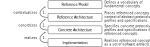
\includegraphics{figures/model-implementation-hierarchy}
  \caption{
    The hierarchical levels comprising the steps from reference models to their software implementation, going from highly abstract to entirly concrete.
    Reference models define fundamental concepts, reference architectures adds abstracts limits to how they may be used together, concrete architectures makes those limits realizable in the real world, and implementations do realize all above levels in practice.
  }
  \label{fig:model-implementation-hierarchy}
\end{figure}

\subsection{Notational Conventions}
\label{sec:introduction:conventions}

\subsubsection{Diagrams}

A box with a name inside it denotes a named \GlossaryHyperRef{entity}{entity-model}.
A named arrow between boxes denotes the \GlossaryHyperRef{relation}{relation-model} implied by the name.
If a named arrow has an associated positive integer or range, the relation is to be considered as extending to the number of unique entities indicated by that integer or range.
A range is denoted by $x..y$, where $x$ and $y$ are positive integers and $x<y$.
Omitting $y$ when using the range notation means that the range is infinite from $x$.
A box being inside another box means that it is owned by the containing box.
See Figure \ref{fig:model-implementation-hierarchy} for an example of this graphical notation being used.

Note that this document does \textit{not} define an Arrowhead profile for SysML \cite{omg2019sysml}, or any other modelling language.
The concepts outlined here should corrsepond to the entities and relations defined by any such profiles, however.

\subsubsection{References}

Square brackets around numbers (e.g. \cite{delsing2017iot}) are references to the reference list in Section \ref{sec:references}.
The number within the brackets of any given reference corresponds to the entry with the same number in the reference list.

\subsubsection{Requirements}

Use of the words \textbf{must}, \textbf{must not}, \textbf{required}, \textbf{should}, \textbf{should not}, \textbf{recommended}, \textbf{may}, and \textbf{optional} are to be interpreted as follows when used in this document: \textbf{must} and \textbf{required} denote absolute requirements that must be adhered to for a described entity to be considered as compliant to this reference model; \textbf{must not} denotes an absolute prohibition; \textbf{should}, \textbf{should not} and \textbf{recommended} denote recommendations that should be deviated from only if special circumstances make it relevant; and, finally, \textbf{may} and \textbf{optional} denote something being truly optional.
These word definitions are derived from and are meant to capture what is outlined in RFC 2119 \cite{bradner1997keywords}.

\subsection{Relationships to Other Documents}
\label{sec:introduction:relationships}

The reference model outlined in this document is based on the following works, in order of precedence:

\begin{enumerate}
\item \textit{RAMI4.0} \cite{adolphs2016reference}, which outlines a ontological and architectural view of Industry 4.0.
As RAMI4.0 is a reference \textit{architecture} rather than a reference \textit{model}, however, its 5\textsuperscript{th} section is disregarded and its remaining sections treated as if being a reference model.
This delimitation excludes the ``architectural layers'', ``life-cycle \& value-stream'' phases and ``hierarchical levels'' of RAMI4.0.

\item \textit{SOA-RM} \cite{mackenzie2006reference}, which provides a standardized definition of SOA.
While RAMI4.0 does not include SOA-RM in its reference list, it does mention the standard and requires that all communications adhere to SOA principles. 

\item \textit{Prior work directly concerned with Arrowhead}.
This significantly includes \textit{IoT Automation: Arrowhead Framework} \cite{delsing2017iot}, which was written to provide a comprehensive overview of the framework.

\end{enumerate}

You are not assumed to have read any of the above documents prior to reading this.
Concepts derived from the above sources are reiterated in this document as necessary.

\subsection{Section Overview}
\label{sec:introduction:sections}

\begin{itemize}[leftmargin=3cm,rightmargin=0pt,labelwidth=2cm,labelsep=0pt,itemindent=0pt,parsep=0.1cm,topsep=0.1cm,align=left]

%\item[Section \ref{sec:introduction}]
%This section.

\item[Section \ref{sec:arrowhead}]
An informal overview of Arrowhead, serving both to provide a workable summary of the framework and to prepare readers for better understanding Section \ref{sec:model}.

\item[Section \ref{sec:model}]
The formal and normative description of Arrowhead.

\item[Section \ref{sec:conformance}]
A brief list of requirements, meant to help determine whether or not a given system is conforming to this document.

\item[Section \ref{sec:glossary}]
Lists all significant terms referred to or defined in this document in alphabetical order.

\item[Section \ref{sec:references}]
Lists references to publications referred to in this document.

\item[Section \ref{sec:revision}]
Records the history of changes made to this document.

\end{itemize}


\section{Certificate Profiles}
\label{sec:profiles}
% Copyright (c) 2021 Eclipse Arrowhead Project
%
% This program and the accompanying materials are made available under the
% terms of the Eclipse Public License 2.0 which is available at
% http://www.eclipse.org/legal/epl-2.0.
%
% SPDX-License-Identifier: EPL-2.0

There are eight certificate profiles defined in this document, depicted in the following diagram:

\begin{figure}[ht!]
  \centering
  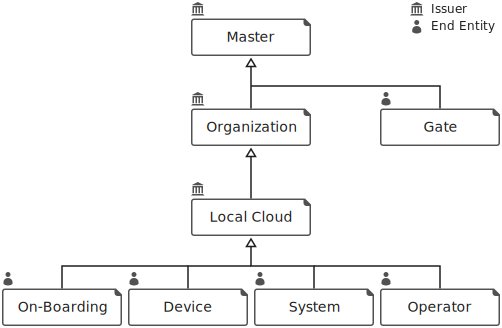
\includegraphics[scale=0.8]{figures/profile-hierarchy}
  \caption{
    Hierarchy of X.509 Profiles
  }
  \label{fig:profile-hierarchy}
\end{figure}

Each diagram box represents a profile.
The arrows in the diagram are to be read as "issued by", meaning that the every certificate adhering to the profile from which the arrow extends must be issued (signed) by a certificate with the profile pointed to.

In this section, we begin by considering the X.509 format itself, after which we outline the Master, Gate, Organization, Local Cloud, On-Boarding, Device, System and Operator profiles.
Each profile is described in terms of its (a) purpose, (b) issuer, (c) subject name and (d) extensions.
The details included in this section are intended to be enough to allow for the correct parameterization of certificates, but are unlikely to be sufficient for implementing software for handling them.
If the latter is relevant, please refer to RFC 5280, X.509, X.501, X.690 and ASN.1.

\subsection{Certificate Format}

The ASN.1 syntax of the third version of the X.509 certificate format is defined in as follows in RFC 5280:

\begin{verbatim}
    Certificate ::= SEQUENCE {
        tbsCertificate       TBSCertificate,
        signatureAlgorithm   AlgorithmIdentifier,
        signatureValue       BIT STRING
    }

    TBSCertificate ::= SEQUENCE {
        version         [0]  EXPLICIT Version DEFAULT v1,
        serialNumber         INTEGER,
        signature            AlgorithmIdentifier,
        issuer               Name,
        validity             Validity,
        subject              Name,
        subjectPublicKeyInfo SubjectPublicKeyInfo,
        issuerUniqueID  [1]  IMPLICIT UniqueIdentifier OPTIONAL,
        subjectUniqueID [2]  IMPLICIT UniqueIdentifier OPTIONAL,
        extensions      [3]  EXPLICIT Extensions OPTIONAL
    }
\end{verbatim}

The \texttt{Certificate} structure itself consists only of a \texttt{TBSCertificate}, a signature algorithm identifier and a concrete signature.
The signature is meant to be produced by the issuer of the certificate and serves to protect the integrity of the certificate under the assumption that the issuer is trusted.
All data protected by the signature is collected in the \texttt{TBSCertificate}, the fields of which are described in the following subsections.

\subsubsection{\texttt{version}}

X.509 version of the certificate.
Only \texttt{v3(2)} supports certificate extensions, which \textit{must} be used by all profiles described in this document.
Supporting \texttt{v1(0)} and \texttt{v2(1)} at all is \textit{optional}.

\subsubsection{\texttt{serialNumber}}

A positive integer of no more than 20 octets uniquely assigned by the issuer of the certificate.

\textbf{Security recommendation}.
The serial number should be exactly 20 octets long and be produced by a cryptographic random number generator.
This serves both to (A) make the certificate more resistant to collision attacks and (B) to prevent the serial number from leaking important details about the certificate issuer, such as how many certificates it has issued, how long the signing process took, and so on.
If certificate size would be a major concern, for example when certificates are used by significantly constrained devices, fewer octets \textit{may} be used.
Note that the serial number is signed and must be positive, which means that the most significant bit of its first ASN.1 BER \texttt{INTEGER} octet must be 0.

\subsubsection{\texttt{signature}}

Identifies the signature suite used to produce the \texttt{signatureValue} in the enclosing \texttt{Certificate}, as well as any parameters made relevant by the suite.
Examples of suites could be \textit{RSA with SHA256} or \textit{ED25519}.
This field must contain the same suite as the \texttt{signatureAlorithm} field in the enclosing \texttt{Certificate}, as described in the beginning of Section 2.1.

See Section 3 for information about selecting cryptographic algorithms.

\subsubsection{\texttt{issuer}}

The DN of the issuer of the certificate in question.
More specifically, this field contains an exact copy of the \texttt{subject} field of Section 2.1.6 from the certificate of its issuer, or a copy of the \texttt{issuer} field of the same certificate if it is self-signed.

\subsubsection{\texttt{validity}}

The period during which the certificate \textit{may} remain active and its issuer is bound to know whether or not the certificate has been revoked or not.
Denoted as a duration between two timestamps, \texttt{notBefore} and \texttt{notAfter}, as show below.

\begin{verbatim}
Validity ::= SEQUENCE {
    notBefore   Time,
    notAfter    Time
}

Time ::= CHOICE {
    utcTime     UTCTime,
    generalTime GeneralizedTime
}
\end{verbatim}

For each of these two dates, the date in question \textit{must} be encoded as a \texttt{UTCTime} if its year is less than or equal to 2049, or as a \texttt{GeneralizedTime} if the year is equal to or greater than 2050.
See Section 4.1.2.5 of RFC 5280 for more details.

The time span denoted by this field \textit{should} be shorter than the expected lifetime of the entity owning it, typically significantly shorter, if provisions exist for renewing it during its lifetime.
More specific recommendations will be published in other documents of the Eclipse Arrowhead project.

\subsubsection{\texttt{subject}}

The DN used to describe the owner of the certificate.
The field is defined as follows:

\begin{verbatim}
Name ::= CHOICE {
    rdnSequence RDNSequence
}

RDNSequence ::= SEQUENCE OF RelativeDistinguishedName

RelativeDistinguishedName ::= SET SIZE (1..MAX) OF AttributeTypeAndValue

AttributeTypeAndValue ::= SEQUENCE {
    type  AttributeType,
    value AttributeValue
}

AttributeType ::= OBJECT IDENTIFIER

-- Concrete type determined by associated \texttt{AttributeType}.
-- In our case that type will always be \texttt{DirectoryString}.
AttributeValue ::= ANY

DirectoryString ::= CHOICE {
     teletexString   TeletexString   (SIZE (1..MAX)),
     printableString PrintableString (SIZE (1..MAX)),
     universalString UniversalString (SIZE (1..MAX)),
     utf8String      UTF8String      (SIZE (1..MAX)),
     bmpString       BMPString       (SIZE (1..MAX)) 
}
\end{verbatim}

The below `AttributeType`s \textit{must} be supported by compliant software implementations, as required by RFC 5280.
Supporting them means that that their OIDs are known to be associated with values of type \texttt{DirectoryString}, as defined above.
Failing to support them means that the certificate validation procedure of RFC 5280, Section 6, cannot be executed.
See RFC 5280 Section 4.1.2.4 for more attributes that \textit{should} be supported.

\vspace*{0.5cm}
\noindent\begin{tabularx}{\textwidth}{| p{5cm} | p{3cm} | X |} \hline
\rowcolor{gray!33} Attribute Type & Abbreviation & OID \\ \hline

Common Name                       & \texttt{CN}  & \texttt{2.5.4.3} \\ \hline
Country                           & \texttt{C}   & \texttt{2.5.4.6}  \\ \hline
Distinguished Name Qualifier      & \texttt{DN}  & \texttt{2.5.4.46} \\ \hline
Domain Component                  & \texttt{DC}  & \texttt{0.9.2342.19200300.100.1.25} \\ \hline
Organization                      & \texttt{O}   & \texttt{2.5.4.10} \\ \hline
Organizational Unit               & \texttt{OU}  & \texttt{2.5.4.11} \\ \hline
Serial Number                     & \texttt{SN}  & \texttt{2.5.4.5} \\ \hline
State or Province Name            & \texttt{ST}  & \texttt{2.5.4.8} \\ \hline

\end{tabularx}
\vspace*{0.5cm}

Every certificate \textit{must} contain at least one \texttt{subject} \textit{Distinguished Name Qualifier} (\texttt{DN}).
It \textit{should} only contain one.
It \textit{should} be encoded as a \texttt{PrintableString}.
The rightmost (i.e. least significant) such identifies the profile of the certificate.
The identifiers are as follows:

\vspace*{0.5cm}
\noindent\begin{tabularx}{\textwidth}{| p{3cm} | X |} \hline
\rowcolor{gray!33} X.509 Profile  & Distinguished Name Qualifier (\texttt{DN}) \\ \hline

Master                            & \texttt{ma} \\ \hline
Gate                              & \texttt{ga} \\ \hline
Organization                      & \texttt{or} \\ \hline
Local Cloud                       & \texttt{lo} \\ \hline
On-Boarding                       & \texttt{on} \\ \hline
Device                            & \texttt{de} \\ \hline
System                            & \texttt{sy} \\ \hline
Operator                          & \texttt{op} \\ \hline

\end{tabularx}
\vspace*{0.5cm}

In addition, each certificate \textit{must} contain at least one \texttt{subject} \textit{Common Name} (\texttt{CN}) that is a valid DNS label (https://datatracker.ietf.org/doc/html/rfc1035\#section-2.3.1) of no more than 62 characters.
It \textit{should} only contain one \texttt{CN}.
It \textit{should} be encoded as a \texttt{PrintableString}.
The rightmost (i.e. least significant) such contains the name, or \textit{alias}, meant to be used by humans when referring to the certificate.
While names \textit{may} use up to 62 characters, we \textit{recommend} the use of 10 to 20 character long lowercase identifiers, such as \texttt{51e41vjoxq}, produced with secure random number generators.
Randomized identifiers hide details that otherwise would become accessible to adversaries with certificate copies, such as how many certificates have been issued, the type of machines they are associated with, and so on.
The \texttt{CN} field value \textit{must}, furthermore, be unique among all certificates issued by the same CA with same Distinguished Name Qualifier (\texttt{DN}).
It \textit{should not} be derived from a portion of the \texttt{serialNumber} of the same certificate.

The \texttt{CN} is meant to help humans refer to specific certificates, they \textit{should not} be used as primary references by machines.
See Section 4 for a discussion about machine certificate references.

\subsubsection{\texttt{subjectPublicKeyInfo}}

The public key of the subject, as well as the identity of the algorithm associated with it.
The field is defined as follows.

\begin{verbatim}
SubjectPublicKeyInfo ::= SEQUENCE {
    algorithm        AlgorithmIdentifier,
    subjectPublicKey BIT STRING
}
\end{verbatim}

See Section 3 for information about selecting cryptographic algorithms.

\subsubsection{\texttt{issuerUniqueID} and \texttt{subjectUniqueID}}

Optional identifiers uniquely associated with the issuer or subject of the certificate.

These fields \textit{must not} be used.
See Section 4 for a discussion about certificate identification.

\subsubsection{\texttt{extensions}}

A list of certificate extensions, as defined below.

\begin{verbatim}
Extensions ::= SEQUENCE SIZE (1..MAX) OF Extension

Extension  ::= SEQUENCE {
    extnID     OBJECT IDENTIFIER,
    critical   BOOLEAN DEFAULT FALSE,
    extnValue  OCTET STRING
}
\end{verbatim}

RFC 5280 explicitly outlines 17 different X.509 extensions, listed by category below.

\vspace*{0.35cm}
\noindent\begin{tabularx}{\textwidth}{| p{4.5cm} | p{2.3cm} | X |} \hline
\rowcolor{gray!33} Extension    & \texttt{extnID} (OID) & Brief Description \\ \hline

\multicolumn{3}{| l |}{\textbf{Identifier Extensions}} \\ \hline
Authority Key Identifier        & \texttt{2.5.29.35}          & Identifier uniquely associated with certificate issuer. \\ \hline
Subject Key Identifier          & \texttt{2.5.29.14}          & Identifier uniquely associated with certificate subject. \\ \hline
\multicolumn{3}{| l |}{\textbf{Key Usage Extensions}} \\ \hline
Key Usage                       & \texttt{2.5.29.15}          & Public key usage restrictions. \\ \hline
Extended Key Usage              & \texttt{2.5.29.37}          & Additional public key usage restrictions. \\ \hline
\multicolumn{3}{| l |}{\textbf{Policy Extensions}} \\ \hline
Certificate Policies            & \texttt{2.5.29.32}          & List of policies accepted by the certificate subject. \\ \hline
Policy Mappings                 & \texttt{2.5.29.33}          & List of policy equivalence relations. \\ \hline
Policy Constraints              & \texttt{2.5.29.36}          & Policy validation constraints (e.g. policy X must be accepted). \\ \hline
Inhibit \texttt{anyPolicy}      & \texttt{2.5.29.54}          & Policy validation constraint related to use of \texttt{anyPolicy}. \\ \hline
\multicolumn{3}{| l |}{\textbf{Name Extensions}} \\ \hline
Subject Alternative Name        & \texttt{2.5.29.17}          & Additional names associated with the certificate subject. \\ \hline
Issuer Alternative Name         & \texttt{2.5.29.18}          & Additional names associated with the certificate issuer. \\ \hline
Name Constraints                & \texttt{2.5.29.30}          & List of subject name restrictions for issued certificates. \\ \hline
\multicolumn{3}{| l |}{\textbf{CRL Extensions}} \\ \hline
CRL Distribution Points         & \texttt{2.5.29.31}          & List of where relevant CRLs can be found. \\ \hline
Freshest CRL                    & \texttt{2.5.29.46}          & List of where delta CRLs can be found. \\ \hline
\multicolumn{3}{| l |}{\textbf{Information Extensions}} \\ \hline
Authority Information Access    & \texttt{1.3.6.1.5. 5.7.1.1}  & List of where issuer information and services can be found. \\ \hline
Subject Information Access      & \texttt{1.3.6.1.5. 5.7.1.11} & List of where subject information and services can be found. \\ \hline
\multicolumn{3}{| l |}{\textbf{Other Extensions}} \\ \hline
Subject Directory Attributes    & \texttt{2.5.29.9}           & Additional subject identification attributes (e.g. nationality). \\ \hline
Basic Constraints               & \texttt{2.5.29.19}          & Description of where a certificate belongs in its CA hierarchy. \\ \hline

\end{tabularx}
\vspace*{0.35cm}

Each category of extensions is described in the following subsections.

\paragraph{Identifier Extensions}

The \textbf{Authority Key Identifier} and \textbf{Subject Key Identifier} extensions are used to identify the public key of the issuer and subject of a given certificate, respectively.
The extensions are defined as follows:

\begin{verbatim}
-- Required for all but self-signed CA certificates (root CAs).
AuthorityKeyIdentifier ::= SEQUENCE {
    keyIdentifier             [0] KeyIdentifier           OPTIONAL, -- Required.
    authorityCertIssuer       [1] GeneralNames            OPTIONAL, -- Should not be used.
    authorityCertSerialNumber [2] CertificateSerialNumber OPTIONAL  -- Should not be used.
}

-- Required for all but end entity certificates.
SubjectKeyIdentifier ::= KeyIdentifier

KeyIdentifier ::= OCTET STRING
\end{verbatim}

RFC 5280 \textit{requires} that \texttt{AuthorityKeyIdentifier} extension is included in all CA certificates except for self-signed such.
The \texttt{keyIdentifier} of the \texttt{AuthorityKeyIdentifier} extension of a given certificate \textit{must} match the \texttt{SubjectKeyIdentifier} of its issuer's certificate, or \textit{may} be omitted if the certificate is self-signed.
Use of the \texttt{authorityCertIssuer} and \texttt{authorityCertSerialNumber} fields of \texttt{AuthorityKeyIdentifier} is \textit{not recommended}.
If a self-signed certificate leaves the \texttt{authorityCertIssuer} and \texttt{authorityCertSerialNumber} fields unspecified, it may omit the \texttt{AuthorityKeyIdentifier} extension entirely.
RFC 5280 further \textit{requires} that all but end entity certificates use the \texttt{SubjectKeyIdentifier} extension.
Its value \textit{should} be the the cryptographic hash of the \texttt{subjectPublicKey} value (excluding the tag, length, and number of unused bits) of the \texttt{subjectPublicKeyInfo} field.
See Section 3 for a discussion about what hash algorithms to use.
The extensions \textit{must not} be marked as critical.

\paragraph{Key Usage Extensions}

The \textbf{Key Usage} and \textbf{Extended Key Usage} extensions are defined as follows:

\begin{verbatim}
KeyUsage ::= BIT STRING {
    digitalSignature (0),
    nonRepudiation   (1), -- Also known as \texttt{contentCommitment}.
    keyEncipherment  (2),
    dataEncipherment (3),
    keyAgreement     (4),
    keyCertSign      (5),
    cRLSign          (6),
    encipherOnly     (7),
    decipherOnly     (8)
}

ExtKeyUsageSyntax ::= SEQUENCE SIZE (1..MAX) OF KeyPurposeId

KeyPurposeId ::= OBJECT IDENTIFIER
\end{verbatim}

The \texttt{KeyUsage} extension is a set of bit flags indicating various ways in which a certificate \textit{must} only be used.
Please refer to RFC 5280 Section 4.2.1.3 for descriptions of each bit flag.
The extension \textit{must} be used in all certificates and \textit{must} be marked as critical.
How to set it is outlined in the section specific to each particular certificate profile.

The \texttt{ExtKeyUsageSyntax} extension has the same purpose, but is open-ended in the sense that it allows for any OID to be used as an indication of what a certain certificate \textit{may} be used for.
RFC 5280 lists six such purpose identifiers, out of which two has particular bearing on this document, namely the \texttt{serverAuth} (OID \texttt{1.3.6.1.5.5.7.3.1}) and \texttt{clientAuth} (OID \texttt{1.3.6.1.5.5.7.3.2}) identifiers, which indicate that the certificate holder must be able to respond to TLS server and client authorization requests, respectively.
The extension \textit{must} be used in all end entity certificates, as well in the certificates of the CAs that handle CSRs directly via network application interfaces.
The \texttt{serverAuth} and \texttt{clientAuth} identifiers \textit{must} be included.
The extension \textit{should not} be marked as \textit{critical}.
Other purpose identifiers \textit{may} be used.

\paragraph{Policy Extensions}

In the context of X.509 and RFC 5280, a \textit{policy} is a legal document that binds the owner of a certificate, and, potentially, all certificates issued by that certificate, to certain legal obligations.
The four policy extensions defined by RFC 5280 \textit{may} be used to ensure that every certificate in a given certificate chain have accepted some policies of concern.
Please refer to RFC 5280 for more details about these extensions.

\paragraph{Name Extensions}

The \textbf{Subject Alternative Name} and \textbf{Issuer Alternative Name} allows for additional identities to be associated with a given \texttt{subject} or \texttt{issuer} name.
Such additional identities significantly include DNS names, IP addresses and e-mail addresses.
For example, given that some system receives a signed message and the certificate associated with that signature, the system can verify that it received the message via one of the identities listed as subject alternative name in that certificate.
The extensions are defined as follows:

\begin{verbatim}
SubjectAltName ::= GeneralNames
IssuerAltName  ::= GeneralNames

GeneralNames ::= SEQUENCE SIZE (1..MAX) OF GeneralName

GeneralName ::= CHOICE {
    otherName                 [0] OtherName,
    rfc822Name                [1] IA5String,
    dNSName                   [2] IA5String,
    x400Address               [3] ORAddress,
    directoryName             [4] Name,
    ediPartyName              [5] EDIPartyName,
    uniformResourceIdentifier [6] IA5String,
    iPAddress                 [7] OCTET STRING,
    registeredID              [8] OBJECT IDENTIFIER
}
\end{verbatim}

The \texttt{SubjectAltName} extension \textit{must} be used by all end entity certificates and \textit{must} identify at least one DNS name, IP address or other relevant identifier useful for contacting the certificate owner.
The extension \textit{must} also be used for CA certificates that handles CSRs directly via network application interfaces.
Use of the \texttt{IssuerAltName} is \textit{not recommended}.
Both extensions \textit{should} be marked as non-critical.

\textbf{Security recommendation}.
All names appearing in a \texttt{SubjectAltName} extension \textit{should} be randomized, by which we mean that every name is formulated such that an adversary can derive as little information as possible from it.
In the case of an IP address, this means that a larger address space is preferred (e.g. 10.0.0.0/8 rather than 192.168.0.0/16) and that addresses are assigned randomly rather than sequentially.
In the case of DNS names, this means that no serially assigned identifiers are used and that no human-readable descriptors of sensitive places or things are part of the name.
See Section 7 for a discussion about the use of DNS in the context of Arrowhead.

The \textbf{Name Constraints} extension makes it possible for a CA to restrict the set of values allowed for the \texttt{subject} and \texttt{SubjectAltName} fields in issued certificates.
The extension \textit{should not} be used.
It \textit{must} be marked as critical if used.
Please refer to RFC 5280 Section 4.2.1.10 for more details.

\paragraph{CRL Extensions}

The CRL extensions facilitate a mechanism for revoking certificates that are still valid and distributing information about those revocations.
These extensions \textit{should not} be used to facilitate the revocation of On-Boarding, Device, System and Operator certificates.
They \textit{may} be used for revoking certificates of the other profiles.

Eclipse Arrowhead comes with its own certificate revocation procedure via its \textit{Certificate Authority} system.
Its use is \textit{recommended} for revoking and verifying the validity of On-Boarding, Device, System and Operator certificates.

\paragraph{Information Extensions}

The information extensions allows for various types of data sources or services to be associated with the certificate holder.
These extensions \textit{should not} be used, unless required by a protocol relevant for the revocation of Master, Organization, Gate and Local Cloud certificates.

Eclipse Arrowhead has its own provisions for metadata distribution and service management, via the \textit{Service Registry} system, \textit{Gatekeeper} system, and other.
Those provisions \textit{should} be used.

\paragraph{Other Extensions}

The \textbf{Subject Directory Attributes} allows for arbitrary identification attributes, such as nationality, to be associated with the \texttt{subject} of a certificate.
It \textit{may} be used.
It \textit{must} be marked as non-critical if used.

The \textbf{Basic Constraints} extension allows for it to be denoted whether or not a given certificate belongs to a CA, as well as how many intermediary CAs may exist below it in any given certificate chain.
The extension is defined as follows:

\newpage

\begin{verbatim}
BasicConstraints ::= SEQUENCE {
    cA                BOOLEAN DEFAULT FALSE,
    pathLenConstraint INTEGER (0..MAX) OPTIONAL
}
\end{verbatim}

The extension \textit{must} be used and marked critical by all Arrowhead-compliant certificates.
The \texttt{pathLenConstraint} \textit{must} be set by all CA certificates, but \textit{must not} be set by end entity certificates.

\newpage
\subsection{Master Profile}

A \textit{Master} certificate exists to establish trust between organizations that may want to interconnect their Arrowhead systems.
It does this by issuing \textit{Organization} and \textit{Gate} certificates.
The former enables organizations to set up their own certificate hierarchies while sharing a common CA with other organizations.
The latter kind enables all those organizations to trust a special kind of broker system, which facilitates negotiating connections between organizations.

The Eclipse Arrowhead project \textit{should} maintain an authoritative Master certificate that \textit{may} be used for non-private Arrowhead installations.
Other entities \textit{may} setup and maintain their own Master certificates as needed.

\subsubsection{\texttt{issuer}}

\textit{May} be self-signed or issued by an RFC 5280-compliant CA.

\textbf{Security notice}.
In the case of a Master being issued by a widely trusted World Wide Web CA, entities with the Master in their certificate chains could be made able to serve HTTP(S) traffic to regular web browsers without any additional certificate distribution.
It could also make it possible for improperly configured systems to establish secure connections with unauthorized systems.
Having CAs above a Master provides for new opportunities and new risks at the same time, for which reason it may or may not be desirable.

\subsubsection{\texttt{subject}}

The subject field DN \textit{must} contain the following attributes exactly once, either in the same or different RDNs:

\vspace*{0.5cm}
\noindent\begin{tabularx}{\textwidth}{| p{4cm} | p{2cm} | X |} \hline
\rowcolor{gray!33} Attribute Type & OID               & Value \\ \hline

DN Qualifier (DN)                 & \texttt{2.5.4.46} & \texttt{ma} \\ \hline
Common Name (CN)                  & \texttt{2.5.4.3}  &  Randomized identifier. See Section 2.1.6. \\ \hline

\end{tabularx}
\vspace*{0.5cm}


\subsubsection{\texttt{extensions}}

The following extensions \textit{must} be used and configured as described:

\vspace*{0.5cm}
\noindent\begin{tabularx}{\textwidth}{| p{4cm} | p{2cm} | p{1.2cm} | X |} \hline
\rowcolor{gray!33} Extension & OID                & Critical & Value \\ \hline

Authority Key Identifier     & \texttt{2.5.29.35} & No       & Hash of issuer public key. Omit field if self-signed. See Section 2.1.9.1. \\ \hline
Subject Key Identifier       & \texttt{2.5.29.14} & No       & Hash of subject public key. See Section 2.1.9.1. \\ \hline
Basic Constraints            & \texttt{2.5.29.19} & Yes      & \texttt{cA: true, pathLenConstraint: 2}. See Section 2.1.9.7. \\ \hline
Key Usage                    & \texttt{2.5.29.15} & Yes      & Bits \texttt{keyCertSign(5)} and \texttt{cRLSign(6)} \textit{must} be set. See Section 2.1.9.2. \\ \hline

\end{tabularx}
\vspace*{0.5cm}

If the certificate will be used to automatically respond to CSRs via a network application interface, the following must also be present:

\vspace*{0.5cm}
\noindent\begin{tabularx}{\textwidth}{| p{4cm} | p{2cm} | p{1.2cm} | X |} \hline
\rowcolor{gray!33} Extension & OID                & Critical & Value \\ \hline

Key Usage                    & \texttt{2.5.29.15} & Yes      & Bits \texttt{digitalSignature(0)} and \texttt{keyEncipherment(2)} \textit{must} be set in addition to \texttt{5} and \texttt{6}. See Section 2.1.9.2. \\ \hline
Extended Key Usage           & \texttt{2.5.29.37} & No       & Purposes`serverAuth` and \texttt{clientAuth} \textit{must} be specified. See Section 2.1.9.2. \\ \hline
Subject Alternative Name     & \texttt{2.5.29.17} & No       & At least one IP address, DNS name or other identifier to which CSRs can be sent. See Section 2.1.9.4. \\ \hline

\end{tabularx}
\vspace*{0.5cm}

\newpage
\subsection{Gate Profile}

A \textit{Gate} certificate is associated with a message broker or bus that exists to guarantee delivery of messages between the local clouds of distinct organizations.
Its existence means that such messages can sent over a secure transport.

\subsubsection{\texttt{issuer}}

\textit{Must} be issued by a Master certificate.

\subsubsection{\texttt{subject}}

The subject field DN \textit{must} contain the following attributes exactly once, either in the same or different RDNs:

\vspace*{0.5cm}
\noindent\begin{tabularx}{\textwidth}{| p{4cm} | p{2cm} | X |} \hline
\rowcolor{gray!33} Attribute Type & OID               & Value \\ \hline

DN Qualifier (DN)                 & \texttt{2.5.4.46} & \texttt{ga} \\ \hline
Common Name (CN)                  & \texttt{2.5.4.3}  &  Randomized identifier. See Section 2.1.6. \\ \hline

\end{tabularx}
\vspace*{0.5cm}

\subsubsection{\texttt{extensions}}

The following extensions \textit{must} be used and configured as described:

\vspace*{0.5cm}
\noindent\begin{tabularx}{\textwidth}{| p{4cm} | p{2cm} | p{1.2cm} | X |} \hline
\rowcolor{gray!33} Extension & OID                & Critical & Value \\ \hline

Authority Key Identifier     & \texttt{2.5.29.35} & No       & Hash of issuer public key. See Section 2.1.9.1. \\ \hline
Basic Constraints            & \texttt{2.5.29.19} & Yes      & \texttt{cA: false}. See Section 2.1.9.7. \\ \hline
Key Usage                    & \texttt{2.5.29.15} & Yes      & Bits \texttt{digitalSignature(0)} and \texttt{keyEncipherment(2)} \textit{must} be set. See Section 2.1.9.2. \\ \hline
Extended Key Usage           & \texttt{2.5.29.37} & No       & Purposes \texttt{serverAuth} and \texttt{clientAuth} \textit{must} be specified. See Section 2.1.9.2. \\ \hline
Subject Alternative Name     & \texttt{2.5.29.17} & No       & At least one IP address, DNS name or other identifier through which the system can be reached. See Section 2.1.9.4. \\ \hline

\end{tabularx}
\vspace*{0.5cm}

\newpage
\subsection{Organization Profile}

An \textit{Organization} certificate is maintained by a single organization, allowing it to manage the certificates of its own local clouds.

\subsubsection{\texttt{issuer}}

\textit{Must} be issued by a Master certificate.

\subsubsection{\texttt{subject}}

The subject field DN \textit{must} contain the following attributes exactly once, either in the same or different RDNs:

\vspace*{0.5cm}
\noindent\begin{tabularx}{\textwidth}{| p{4cm} | p{2cm} | X |} \hline
\rowcolor{gray!33} Attribute Type & OID               & Value \\ \hline

DN Qualifier (DN)                 & \texttt{2.5.4.46} & \texttt{or} \\ \hline
Common Name (CN)                  & \texttt{2.5.4.3}  &  Randomized identifier. See Section 2.1.6. \\ \hline

\end{tabularx}
\vspace*{0.5cm}

\subsubsection{\texttt{extensions}}

The following extensions \textit{must} be used and configured as described:

\vspace*{0.5cm}
\noindent\begin{tabularx}{\textwidth}{| p{4cm} | p{2cm} | p{1.2cm} | X |} \hline
\rowcolor{gray!33} Extension & OID                & Critical & Value \\ \hline

Authority Key Identifier     & \texttt{2.5.29.35} & No       & Hash of issuer public key. See Section 2.1.9.1. \\ \hline
Subject Key Identifier       & \texttt{2.5.29.14} & No       & Hash of subject public key. See Section 2.1.9.1. \\ \hline
Basic Constraints            & \texttt{2.5.29.19} & Yes      & \texttt{cA: true, pathLenConstraint: 1}. See Section 2.1.9.7. \\ \hline
Key Usage                    & \texttt{2.5.29.15} & Yes      & Bits \texttt{keyCertSign(5)} and \texttt{cRLSign(6)} \textit{must} be set. See Section 2.1.9.2. \\ \hline

\end{tabularx}
\vspace*{0.5cm}

If the certificate will be used to automatically respond to CSRs via a network application interface, the following must also be present:

\vspace*{0.5cm}
\noindent\begin{tabularx}{\textwidth}{| p{4cm} | p{2cm} | p{1.2cm} | X |} \hline
\rowcolor{gray!33} Extension & OID                & Critical & Value \\ \hline

Key Usage                    & \texttt{2.5.29.15} & Yes      & Bits \texttt{digitalSignature(0)} and \texttt{keyEncipherment(2)} \textit{must} be set in addition to \texttt{5} and \texttt{6}. See Section 2.1.9.2. \\ \hline
Extended Key Usage           & \texttt{2.5.29.37} & No       & Purposes`serverAuth` and \texttt{clientAuth} \textit{must} be specified. See Section 2.1.9.2. \\ \hline
Subject Alternative Name     & \texttt{2.5.29.17} & No       & At least one IP address, DNS name or other identifier to which CSRs can be sent. See Section 2.1.9.4. \\ \hline

\end{tabularx}
\vspace*{0.5cm}

\newpage
\subsection{Local Cloud Profile}

An \textit{Local Cloud} certificate is maintained by a single local cloud, enabling it to issue end entity certificates for on-boarding and on-boarded devices, as well as for systems and operators.

\subsubsection{\texttt{issuer}}

\textit{Must} be issued by an Organization certificate.

\subsubsection{\texttt{subject}}

The subject field DN \textit{must} contain the following attributes exactly once, either in the same or different RDNs:

\vspace*{0.5cm}
\noindent\begin{tabularx}{\textwidth}{| p{4cm} | p{2cm} | X |} \hline
\rowcolor{gray!33} Attribute Type & OID               & Value \\ \hline

DN Qualifier (DN)                 & \texttt{2.5.4.46} & \texttt{lo} \\ \hline
Common Name (CN)                  & \texttt{2.5.4.3}  &  Randomized identifier. See Section 2.1.6. \\ \hline

\end{tabularx}
\vspace*{0.5cm}

\subsubsection{\texttt{extensions}}

The following extensions \textit{must} be used and configured as described:

\vspace*{0.5cm}
\noindent\begin{tabularx}{\textwidth}{| p{4cm} | p{2cm} | p{1.2cm} | X |} \hline
\rowcolor{gray!33} Extension & OID                & Critical & Value \\ \hline

Authority Key Identifier     & \texttt{2.5.29.35} & No       & Hash of issuer public key. See Section 2.1.9.1. \\ \hline
Subject Key Identifier       & \texttt{2.5.29.14} & No       & Hash of subject public key. See Section 2.1.9.1. \\ \hline
Basic Constraints            & \texttt{2.5.29.19} & Yes      & \texttt{cA: true, pathLenConstraint: 0}. See Section 2.1.9.7. \\ \hline
Key Usage                    & \texttt{2.5.29.15} & Yes      & Bits \texttt{keyCertSign(5)} and \texttt{cRLSign(6)} \textit{must} be set. See Section 2.1.9.2. \\ \hline

\end{tabularx}
\vspace*{0.5cm}

If the certificate will be used to automatically respond to CSRs via a network application interface, the following must also be present:

\vspace*{0.5cm}
\noindent\begin{tabularx}{\textwidth}{| p{4cm} | p{2cm} | p{1.2cm} | X |} \hline
\rowcolor{gray!33} Extension & OID                & Critical & Value \\ \hline

Key Usage                    & \texttt{2.5.29.15} & Yes      & Bits \texttt{digitalSignature(0)} and \texttt{keyEncipherment(2)} \textit{must} be set in addition to \texttt{5} and \texttt{6}. See Section 2.1.9.2. \\ \hline
Extended Key Usage           & \texttt{2.5.29.37} & No       & Purposes`serverAuth` and \texttt{clientAuth} \textit{must} be specified. See Section 2.1.9.2. \\ \hline
Subject Alternative Name     & \texttt{2.5.29.17} & No       & At least one IP address, DNS name or other identifier to which CSRs can be sent. See Section 2.1.9.4. \\ \hline

\end{tabularx}
\vspace*{0.5cm}

\newpage
\subsection{On-Boarding Profile}

An \textit{On-Boarding} certificate allows for a device in an Arrowhead local cloud to request a new device certificate.
It is used both or either to provision new devices and/or to facilitate renewal of certificates as they are about to expire.
Certificates adhering to this profile \textit{must} only be provided to devices known or assumed to be trustworthy.

\subsubsection{\texttt{issuer}}

\textit{Must} be issued by a Local Cloud certificate.

\subsubsection{\texttt{subject}}

The subject field DN \textit{must} contain the following attributes exactly once, either in the same or different RDNs:

\vspace*{0.5cm}
\noindent\begin{tabularx}{\textwidth}{| p{4cm} | p{2cm} | X |} \hline
\rowcolor{gray!33} Attribute Type & OID               & Value \\ \hline

DN Qualifier (DN)                 & \texttt{2.5.4.46} & \texttt{on} \\ \hline
Common Name (CN)                  & \texttt{2.5.4.3}  &  Randomized identifier. See Section 2.1.6. \\ \hline

\end{tabularx}
\vspace*{0.5cm}

\subsubsection{\texttt{extensions}}

The following extensions \textit{must} be used and configured as described:

\vspace*{0.5cm}
\noindent\begin{tabularx}{\textwidth}{| p{4cm} | p{2cm} | p{1.2cm} | X |} \hline
\rowcolor{gray!33} Extension & OID                & Critical & Value \\ \hline

Authority Key Identifier     & \texttt{2.5.29.35} & No       & Hash of issuer public key. See Section 2.1.9.1. \\ \hline
Basic Constraints            & \texttt{2.5.29.19} & Yes      & \texttt{cA: false}. See Section 2.1.9.7. \\ \hline
Key Usage                    & \texttt{2.5.29.15} & Yes      & Bits \texttt{digitalSignature(0)} and \texttt{keyEncipherment(2)} \textit{must} be set. See Section 2.1.9.2. \\ \hline
Extended Key Usage           & \texttt{2.5.29.37} & No       & Purposes \texttt{serverAuth} and \texttt{clientAuth} \textit{must} be specified. See Section 2.1.9.2. \\ \hline
Subject Alternative Name     & \texttt{2.5.29.17} & No       & At least one IP address, DNS name or other identifier through which the owning device can be reached. See Section 2.1.9.4. \\ \hline

\end{tabularx}
\vspace*{0.5cm}

\newpage
\subsection{Device Profile}

A \textit{Device} certificate allows for a device in an Arrowhead local cloud to request new system certificates.
One system certificate is required for each system a given device intends to run.
Certificates adhering to this profile \textit{must} only be provided to devices known or assumed to be trustworthy.

\subsubsection{\texttt{issuer}}

\textit{Must} be issued by a Local Cloud certificate.

\subsubsection{\texttt{subject}}

The subject field DN \textit{must} contain the following attributes exactly once, either in the same or different RDNs:

\vspace*{0.5cm}
\noindent\begin{tabularx}{\textwidth}{| p{4cm} | p{2cm} | X |} \hline
\rowcolor{gray!33} Attribute Type & OID               & Value \\ \hline

DN Qualifier (DN)                 & \texttt{2.5.4.46} & \texttt{de} \\ \hline
Common Name (CN)                  & \texttt{2.5.4.3}  &  Randomized identifier. See Section 2.1.6. \\ \hline

\end{tabularx}
\vspace*{0.5cm}

\subsubsection{\texttt{extensions}}

The following extensions \textit{must} be used and configured as described:

\vspace*{0.5cm}
\noindent\begin{tabularx}{\textwidth}{| p{4cm} | p{2cm} | p{1.2cm} | X |} \hline
\rowcolor{gray!33} Extension & OID                & Critical & Value \\ \hline

Authority Key Identifier     & \texttt{2.5.29.35} & No       & Hash of issuer public key. See Section 2.1.9.1. \\ \hline
Basic Constraints            & \texttt{2.5.29.19} & Yes      & \texttt{cA: false}. See Section 2.1.9.7. \\ \hline
Key Usage                    & \texttt{2.5.29.15} & Yes      & Bits \texttt{digitalSignature(0)} and \texttt{keyEncipherment(2)} \textit{must} be set. See Section 2.1.9.2. \\ \hline
Extended Key Usage           & \texttt{2.5.29.37} & No       & Purposes \texttt{serverAuth} and \texttt{clientAuth} \textit{must} be specified. See Section 2.1.9.2. \\ \hline
Subject Alternative Name     & \texttt{2.5.29.17} & No       & At least one IP address, DNS name or other identifier through which the device can be reached. See Section 2.1.9.4. \\ \hline

\end{tabularx}
\vspace*{0.5cm}

\newpage
\subsection{System Profile}

A \textit{System} certificate allows for a device in an Arrowhead local cloud to provide the services associated with a particular system, and/or to act as a service consumer.

\subsubsection{\texttt{issuer}}

\textit{Must} be issued by a Local Cloud certificate.

\subsubsection{\texttt{subject}}

The subject field DN \textit{must} contain the following attributes exactly once, either in the same or different RDNs:

\vspace*{0.5cm}
\noindent\begin{tabularx}{\textwidth}{| p{4cm} | p{2cm} | X |} \hline
\rowcolor{gray!33} Attribute Type & OID               & Value \\ \hline

DN Qualifier (DN)                 & \texttt{2.5.4.46} & \texttt{sy} \\ \hline
Common Name (CN)                  & \texttt{2.5.4.3}  &  Randomized identifier. See Section 2.1.6. \\ \hline

\end{tabularx}
\vspace*{0.5cm}

\subsubsection{\texttt{extensions}}

The following extensions \textit{must} be used and configured as described:

\vspace*{0.5cm}
\noindent\begin{tabularx}{\textwidth}{| p{4cm} | p{2cm} | p{1.2cm} | X |} \hline
\rowcolor{gray!33} Extension & OID                & Critical & Value \\ \hline

Authority Key Identifier     & \texttt{2.5.29.35} & No       & Hash of issuer public key. See Section 2.1.9.1. \\ \hline
Basic Constraints            & \texttt{2.5.29.19} & Yes      & \texttt{cA: false}. See Section 2.1.9.7. \\ \hline
Key Usage                    & \texttt{2.5.29.15} & Yes      & Bits \texttt{digitalSignature(0)} and \texttt{keyEncipherment(2)} \textit{must} be set. See Section 2.1.9.2. \\ \hline
Extended Key Usage           & \texttt{2.5.29.37} & No       & Purposes \texttt{serverAuth} and \texttt{clientAuth} \textit{must} be specified. See Section 2.1.9.2. \\ \hline
Subject Alternative Name     & \texttt{2.5.29.17} & No       & At least one IP address, DNS name or other identifier through which the system can be reached. See Section 2.1.9.4. \\ \hline

\end{tabularx}
\vspace*{0.5cm}

\newpage
\subsection{Operator Profile}

An \textit{Operator} certificate allows for a human or computer operator to administer a particular Arrowhead local cloud.

\subsubsection{\texttt{issuer}}

\textit{Must} be issued by a Local Cloud certificate.

\subsubsection{\texttt{subject}}

The subject field DN \textit{must} contain the following attributes exactly once, either in the same or different RDNs:

\vspace*{0.5cm}
\noindent\begin{tabularx}{\textwidth}{| p{4cm} | p{2cm} | X |} \hline
\rowcolor{gray!33} Attribute Type & OID               & Value \\ \hline

DN Qualifier (DN)                 & \texttt{2.5.4.46} & \texttt{op} \\ \hline
Common Name (CN)                  & \texttt{2.5.4.3}  &  Randomized identifier. See Section 2.1.6. \\ \hline

\end{tabularx}
\vspace*{0.5cm}

\subsubsection{\texttt{extensions}}

The following extensions \textit{must} be used and configured as described:

\vspace*{0.5cm}
\noindent\begin{tabularx}{\textwidth}{| p{4cm} | p{2cm} | p{1.2cm} | X |} \hline
\rowcolor{gray!33} Extension & OID                & Critical & Value \\ \hline

Authority Key Identifier     & \texttt{2.5.29.35} & No       & Hash of issuer public key. See Section 2.1.9.1. \\ \hline
Basic Constraints            & \texttt{2.5.29.19} & Yes      & \texttt{cA: false}. See Section 2.1.9.7. \\ \hline
Key Usage                    & \texttt{2.5.29.15} & Yes      & Bits \texttt{digitalSignature(0)} and \texttt{keyEncipherment(2)} \textit{must} be set. See Section 2.1.9.2. \\ \hline
Extended Key Usage           & \texttt{2.5.29.37} & No       & Purposes \texttt{serverAuth} and \texttt{clientAuth} \textit{must} be specified. See Section 2.1.9.2. \\ \hline
Subject Alternative Name     & \texttt{2.5.29.17} & No       & At least one IP address, DNS name or other identifier through which the operator's control system can be reached. See Section 2.1.9.4. \\ \hline

\end{tabularx}
\vspace*{0.5cm}


\section{Algorithms, Key Lengths and Other Security Details}
\label{sec:security}
% Copyright (c) 2021 Eclipse Arrowhead Project
%
% This program and the accompanying materials are made available under the
% terms of the Eclipse Public License 2.0 which is available at
% http://www.eclipse.org/legal/epl-2.0.
%
% SPDX-License-Identifier: EPL-2.0

WChoosing a signature suite for a certificate poorly can lead to severe security vulnerabilities.
We \textit{recommend} that credible information security institutes, such as NIST, ENSIA or IETF, be consulted for making choices about algorithms, key lengths and other relevant security details.

Given that no relevant breakthroughs are made or expected in quantum computing, you \textit{may} chose to follow RFC 7525, which recommends the following four TLS cipher suites:

| Key Exchange | Authentication             | Encryption  | Hash   |
|:-------------|:---------------------------|:------------|:-------|
| DHE          | RSA (2048-bit or 3072-bit) | AES 128 GCM | SHA256 |
| ECDHE        | RSA (2048-bit or 3072-bit) | AES 128 GCM | SHA256 |
| DHE          | RSA (2048-bit or 3072-bit) | AES 256 GCM | SHA384 |
| ECDHE        | RSA (2048-bit or 3072-bit) | AES 256 GCM | SHA384 |

Only the first of the above cipher suites is required to be supported by all TLS 1.3 implementations (RFC 8446, Section 9.1).
Each cipher suite includes a signature suite (the \textit{Authentication} and \textit{Hash} fields).
Adherence to RFC 7525 means that RSA (2048-bit or 3072-bit) with SHA256 or SHA384 is used to sign certificates.
Given that RFC 7525 is trusted, SHA256 and SHA384 \textit{may} be suitable choices for producing certificate identifiers, as discussed in Section 4.

The above recommendations are \textit{general}, in the sense that no particular assumptions are made about the setting in which the device employing the signature or cipher suite is located.
We understand that many Arrowhead installations will involve hardware with limited computational capabilities, which may not be able to handle primitives of the cryptographic strengths we have mentioned.
The Eclipse Arrowhead project will publish summaries of recommendations for such and other settings in the future.

\section{Identifying Certificates and Their Owners}
\label{sec:identification}
% Copyright (c) 2021 Eclipse Arrowhead Project
%
% This program and the accompanying materials are made available under the
% terms of the Eclipse Public License 2.0 which is available at
% http://www.eclipse.org/legal/epl-2.0.
%
% SPDX-License-Identifier: EPL-2.0

The X.509 profiles of this document provide two fields and one extension whose values could be used to identify a particular certificate or its owner.
These are the the `serialNumber` and `subject` fields, as well as the `Subject Key Identifier` extension.
Despite this, they \textit{must not} be used by machines referring to certificates.
The reason for this is that they are all set arbitrarily by the creator of each certificate.
An adversary with a given certificate could create another certificate with the same values, allowing it to masquerade as the owner of the original certificate without knowledge of its private key.

What \textit{should} be used, rather, is either (1) the cryptographic hash of an entire certificate in its DER form (i.e. its fingerprint) or (2) the cryptographic hash of its `subjectPublicKey` value (excluding the tag, length, and number of unused bits) of the `subjectPublicKeyInfo` field, also in its DER form.
While the second of these two identifiers will be equal to the `Subject Key Identifier` for a conformant certificate, it \textit{should not} be generally assumed that a given certificate is conformant.
Both of these hashes include the public key of the certificate owner, which means that it becomes harder for an adversary to create a counterfeit certificate.
We \textit{recommend} that the certificate hash (fingerprint) be generally used as identifier, as it protects the integrity of the entire certificate as opposed to only one field of it.
See Section 3 for details about what hash algorithms to use.


\section{Certificate Life-Cycle Management}
\label{sec:life-cycle}
% Copyright (c) 2021 Eclipse Arrowhead Project
%
% This program and the accompanying materials are made available under the
% terms of the Eclipse Public License 2.0 which is available at
% http://www.eclipse.org/legal/epl-2.0.
%
% SPDX-License-Identifier: EPL-2.0

Certificates must be created, distributed, replaced as they expire and, sometimes, revoked before they expire.
If these tasks are handled without care, it can lead to serious security vulnerabilities.
To help making this handling as rigorous as possible, the Eclipse Arrowhead project provides the \textit{Certificate Authority} system, which, through some other helper systems, provides an infrastructure for managing the certificate life-cycle within local clouds.
We \textit{recommend} that the system be used, or a similarly capable replacement, for all Eclipse Arrowhead installations.

Generally, when certificate life-cycles are managed, we \textit{recommend} that the following be observed:

1. Create each private key on the device that will use it.
2. Use CSRs to avoid moving private keys between devices during certificate issuance.
3. Never make backups or other copies of private keys that can be trivially replaced.
4. Store backups of sensitive private keys offline, if possible.
5. Store active private keys in secure hardware elements, such as TPMs (ISO/IEC 11889).
6. Immediately revoke owned certificates whose private keys are suspected to be compromised.
7. Actively look for and act on revocations in the certificate chains of counter-parties.

The above list is \textit{not} to be considered as being exhaustive.
Adhering to it is not a substitute for consulting independent and credible security experts.
The list is likely to be revised as more experience is gained related to the security of Arrowhead installations.

\section{Authorizing Certificate Owners}
\label{sec:authorization}
% Copyright (c) 2021 Eclipse Arrowhead Project
%
% This program and the accompanying materials are made available under the
% terms of the Eclipse Public License 2.0 which is available at
% http://www.eclipse.org/legal/epl-2.0.
%
% SPDX-License-Identifier: EPL-2.0

While no steps in addition to those in Section 6 of RFC 5280 are mandatory for certificate \textit{validation}, there are additional details made available by our profiles that \textit{should} be used for \textit{authorization} when applicable.
These details are (A) profile identifiers and (B) issuer identities.
For example, if an Arrowhead system provides a service, it \textit{may} be relevant to ensure that any consumer of that service belongs to the same local cloud and is an operator.

We \textit{recommend} that a procedure practically equivalent to the below algorithm, described in pseudo-code, is used when extracting certificate profile identifiers.
The input to the algorithm is an array containing a certificate chain `chain` of a given peer.
The certificate at index 0 of that array is owned by the peer in question, while the remaining certificates represent its issuance hierarchy, in order of issuance from least significant to most.

\begin{verbatim}
function getCertificateProfileIdentifier(chain) {
    if (chain.length == 0) { throw "empty chain"; }

    let dnq = getDNQualifier(chain[0]);
    switch (dnq) {
        case "ma":
            break;
        case "or": case "ga":
            requireProfileSequence(chain[1..], ["ma"]); break;
        case "lo":
            requireProfileSequence(chain[1..], ["or", "ma"]); break;
        case "on": case "de": case "sy": case "op":
            requireProfileSequence(chain[1..], ["lo", "or", "ma"]); break;
        default:
            throw "unexpected DNQualifier";
    }
    return dnq;
}

function requireProfileSequence(chain, identifiers) {
    if (identifiers.length == 0) { return; }
    if (chain.length == 0) { throw "expected additional certificate(s)"; }

    if (getDNQualifier(chain[0]) != identifiers[0]) {
        throw "unexpected certificate profile";
    }

    requireProfileSequence(chain[1..], identifiers[1..]);
}
\end{verbatim}

The `getDNQualifier` function is assumed to extract the `subject` `DN` field, described in Section 2.1.6, of a given certificate.
If several such fields is present in a given certificate, the rightmost (i.e. least significant) must be returned by the function.
The `[1..]` notation is used to describe an array being "sliced" such that a new array is produced containing all but the first element of the original array.
The algorithm asserts that any extracted identifier appears at the expected hierarchical level, apart from extracting the identifier itself.

Testing elements of an issuance hierarchy could be performed by comparing certificate DER representations byte by byte, or by comparing their DER hashes.
The following pseudo-code describes how a service provider could assert that a given peer is a system belonging to a certain local cloud:

\begin{verbatim}
if (getCertificateProfileIdentifier(peer.chain) != "sy" || hash(peer.chain[1]) != hashOfRelevantLocalCloudCertificate) {
    throw "unauthorized";
}
\end{verbatim}

Note that if either of the secure transports TLS or DTLS is used by a given Arrowhead peer, the `post\_handshake\_auth` extension (RFC 8446, Section 4.6.2), must be required in order for both peers of a connection to provide and validate certificates.
The extension \textit{should} always be required when Arrowhead systems communicate.
Use of the `post\_handshake\_auth` extension is referred to as \textit{client authentication} by many software libraries and applications, as the initiating peer, or \textit{client}, is also authenticated by the responding peer, or \textit{server}.

\renewcommand{\bibsection}{\section{References}\label{sec:references}}
\bibliographystyle{arrowhead}
\bibliography{bibliography}

\newpage

\section{Revision History}
\label{sec:revision}

\subsection{Amendments}

\noindent\begin{tabularx}{\textwidth}{| p{1cm} | p{2cm} | p{1.25cm} | X | p{4cm} |} \hline
\rowcolor{gray!33} No. & Date & Version & Subject of Amendments & Author \\ \hline

1 & & & & \\ \hline

\end{tabularx}

\subsection{Quality Assurance}

\noindent\begin{tabularx}{\textwidth}{| p{1cm} | p{2cm} | p{1.25cm} | X |} \hline
\rowcolor{gray!33} No. & Date & Version & Approved by \\ \hline

1 & & & \\ \hline

\end{tabularx}

\end{document}